\documentclass{beamer}


\usepackage{amsmath, fontspec}
\usefonttheme{serif}

\usepackage[document]{ragged2e}
\usepackage{xeCJK}
\setCJKmainfont{SimSun} % 设置中文字体为宋体


\usepackage{beamerthemesplit} % 加载主题宏包
\usetheme{Warsaw} % 选用该主题


%插入图片, 写公式, 画表格等
\usepackage{subfig}
\usepackage{amssymb,mathtools}
\usepackage{amsfonts,booktabs}
\usepackage{lmodern,textcomp}
\usepackage{color}
\usepackage{tikz}
\usepackage[utf8]{inputenc}
\usepackage{natbib}
\usepackage{multicol}
\usepackage{graphicx}
\usepackage{bm}
\usepackage{adjustbox}
%\usepackage{meadia9}  %这个包可以插入视频

\setbeamertemplate{footline}{\hfill\insertframenumber/\inserttotalframenumber} % 页脚为页码
\setbeamertemplate{headline}{}


%%%%%%%%%%%%%%%%%%%%%%%%%%%%%%%%%%%%%%%%%%%%%%%%%%%%%%%%
% 注意这部分代码将全角的逗号句号转换为了半角的逗号句号且半角逗号后面跟了一个空格,要求用xelatex编译,但模板撰写的时候默认用pdflatex,不推荐使用

\catcode`,=\active
\newcommand{,}{, }

\catcode`。=\active
\newcommand{。}{.}

\catcode`:=\active
\newcommand{:}{: }
%%%%%%%%%%%%%%%%%%%%%%%%%%%%%%%%%%%%%%%%%%%%%%%%%%%%%%%%


\begin{document}
	
	%基本信息
	\title{参考最简二足模型的基于一些假设\\与近似的一步内四足模型的理论建立}
	\subtitle{主要由组长姚涵清提供}
	%\subtitle{电磁学荣誉课讨论}
	\author{林海轩}
	\institute{复旦大学物理学系}
	\date{}
	
	%生成标题页
	\begin{frame}
		\titlepage
	\end{frame}
	
	%目录页,代码无需改动
	\begin{frame}
		\tableofcontents
	\end{frame}
	
	
	%%%%%%%%%%%%%%%%%%%%%%%%%%%%%%%%%%%%%%%%%%%%%%%%%%%%%%%%%%%%%%%%%%%%%%%%%%%%%%%%%%%%%%%%%%%%%%%

	\section{事实、符号与约定}
		
	\begin{frame}[plain,c]
		\begin{center}
			\Huge 事实、符号与约定
		\end{center}
	\end{frame}
	
	\begin{frame}
		\frametitle{前提与事实的陈述}
		\begin{enumerate}
			\item 拖地滑行总是发生在后腿,若否则整体打滑,非研究范畴
			\item 能量的耗散总是来源于后腿的摩擦,本模型旨在定量分析一次步态内的运动方程,所以触地损耗不被考量
		\end{enumerate}
	\end{frame}
	
	\begin{frame}
		\frametitle{腿的序号的约定}
		\begin{figure}
			\centering
			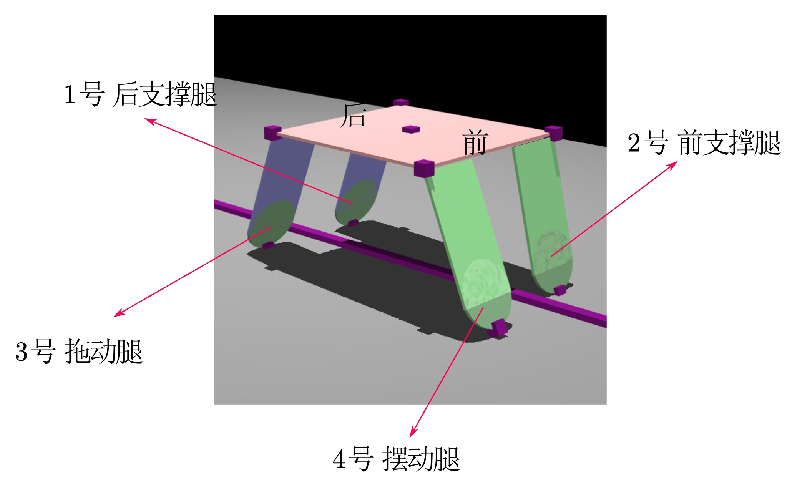
\includegraphics[width=0.95\linewidth]{SomeAppoints}
			\caption*{}
			\label{fig:someappoints}
		\end{figure}
	\end{frame}
	
	\begin{frame}
		\frametitle{左视图}
		\begin{figure}
			\centering
			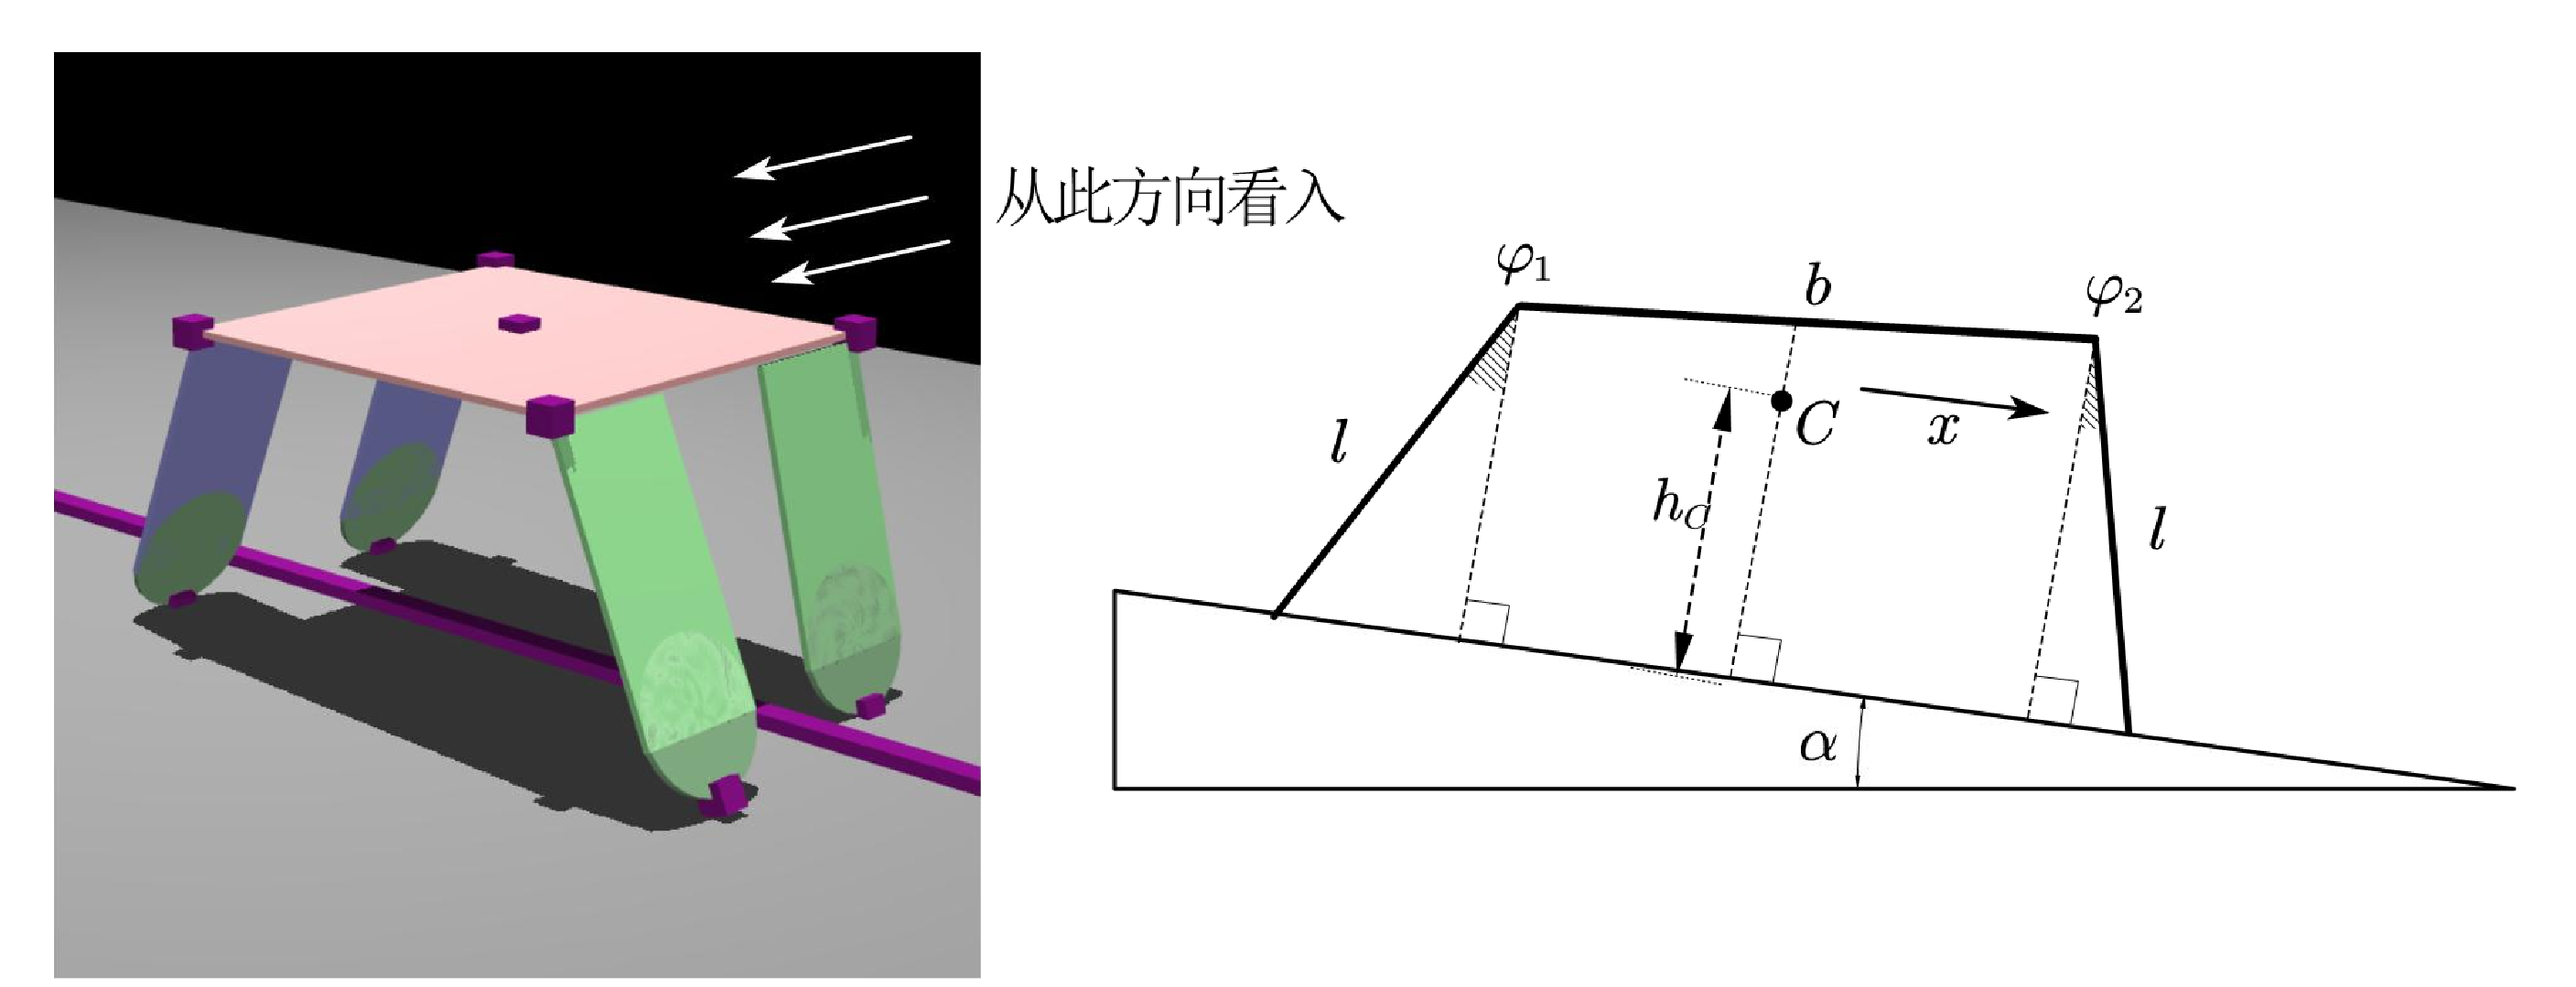
\includegraphics[width=1.1\linewidth]{LeftSee}
			\caption*{}
			\label{fig:leftsee}
		\end{figure}
		\begin{enumerate}
			\item $C$点是质心. 我们假定没有横向的偏移,尽管这略微与事实相悖, 在此基础上设$x$是质心相对坐标原点的位移
			\item $l$, $b$,$h_C$分别是腿长,身长,质心到斜面的垂直高度
			\item $\varphi_1$, $\varphi_2$, $\alpha$分别是后支撑腿1号与垂直斜面的夹角,前支撑腿2号与垂直斜面的夹角,斜面倾角
		\end{enumerate}
	\end{frame}
	
	\begin{frame}
		\frametitle{右视图}
		\begin{figure}
			\centering
			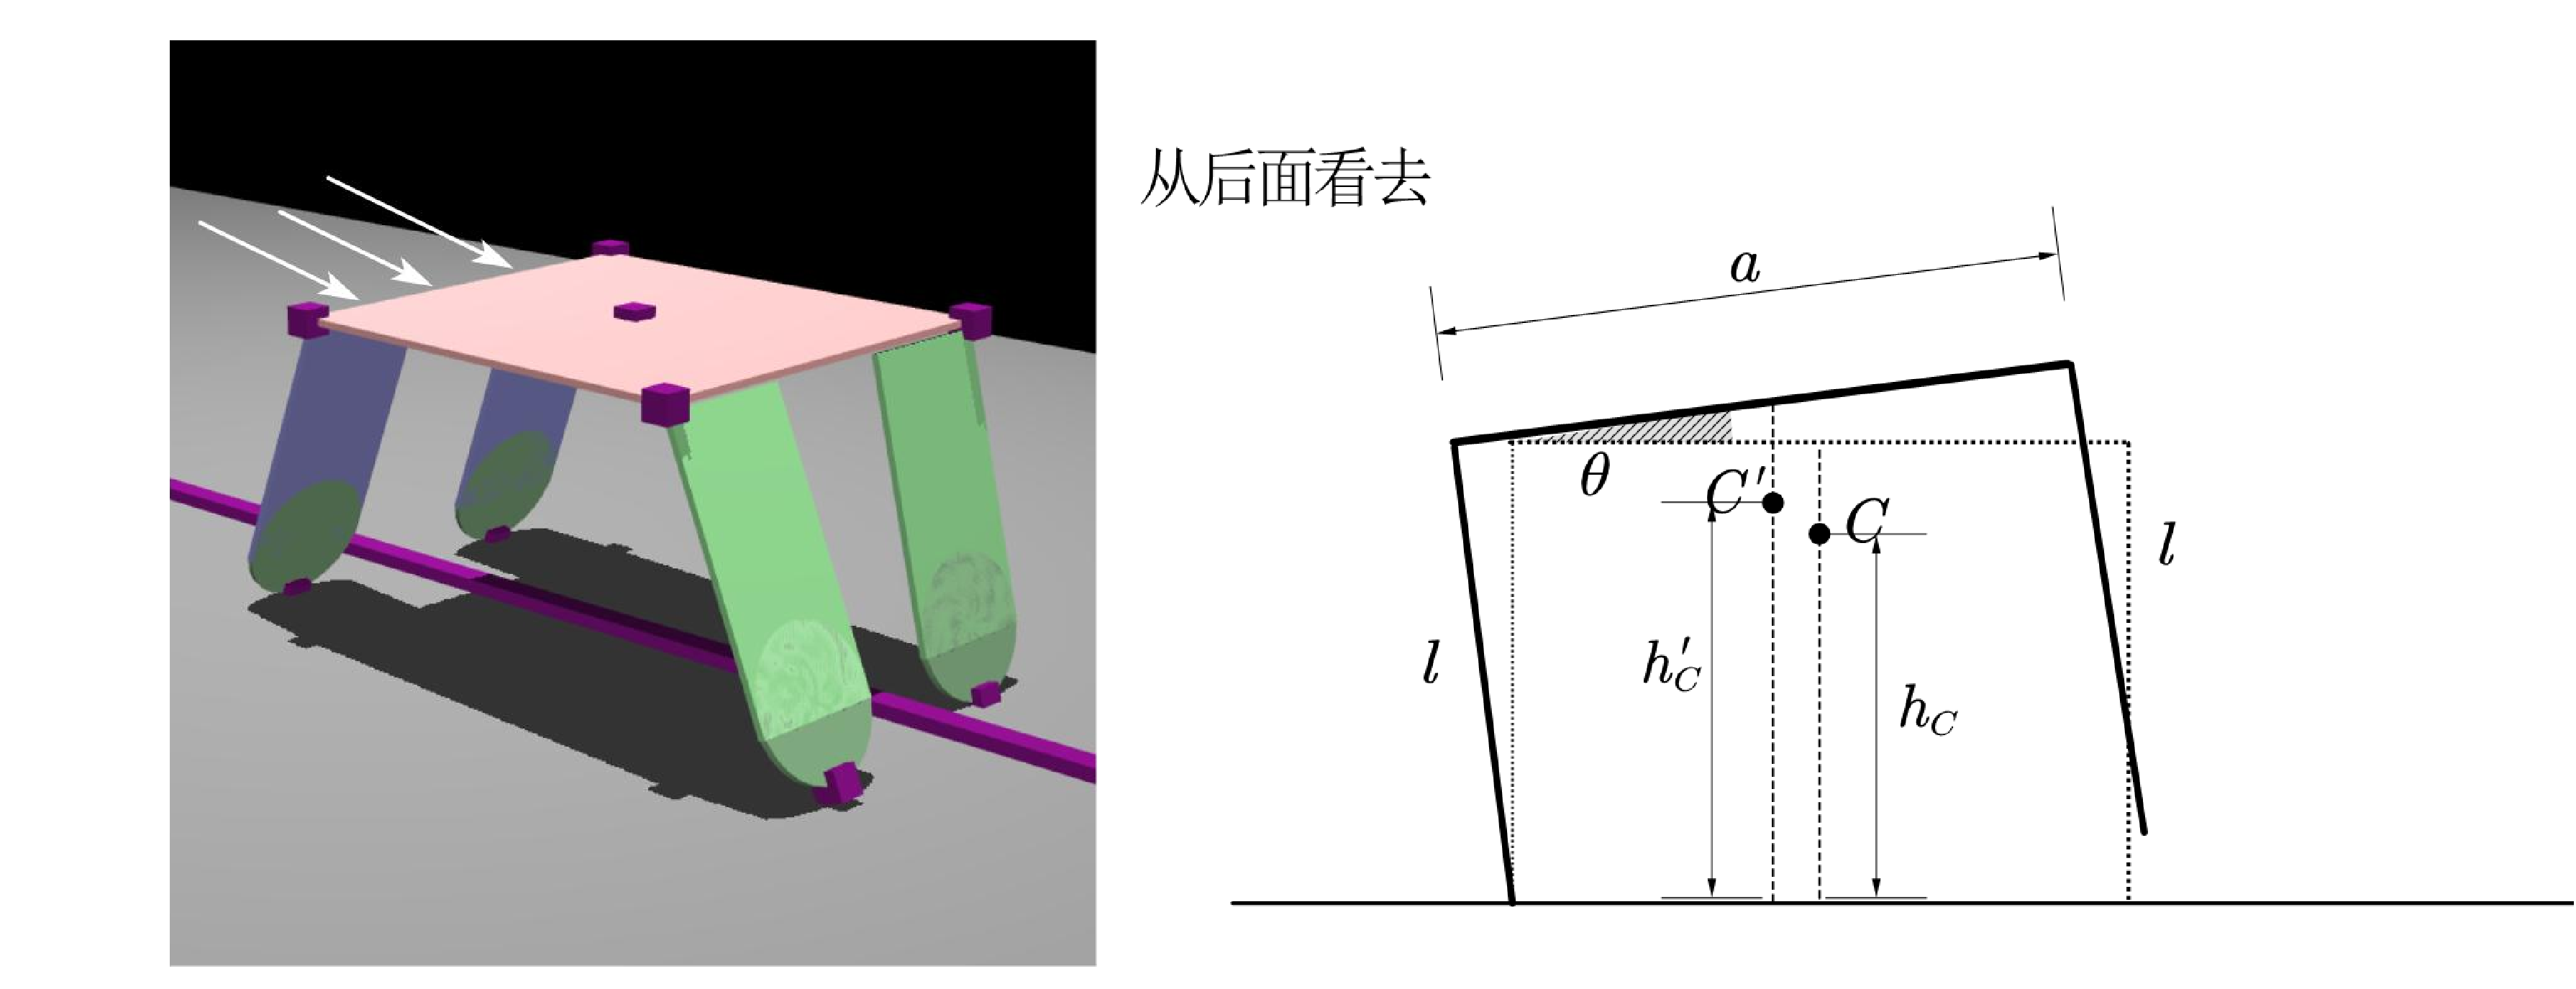
\includegraphics[width=1.1\linewidth]{BehindSee}
			\caption*{}
			\label{fig:behindsee}
		\end{figure}
		\begin{enumerate}
			\item $a$是身子的长度
			\item $\theta$是身子沿$x$轴侧转的角度
			\item 设关节的角量劲度系数为$k$, 关节的平衡位置是$\beta$
		\end{enumerate}
	\end{frame}
	
	\section{各物理量的推导}
	
	\begin{frame}[plain,c]
		\begin{center}
			\Huge 各物理量的推导
		\end{center}
	\end{frame}
	
	\begin{frame}
		\frametitle{势能}
		重力势能为
		$$
		V_G=mg\left[ -x\sin \alpha +\left( h_{C}^{\prime}-h_C \right) \cos \alpha \right] 
		$$
		弹性势能为
		\begin{align*}
			V_k&=\frac{1}{2}k\sum_{i=1}^4{\left( \varphi _i-\beta \right) ^2}\\
			&=\frac{1}{2}k\left[ \left( \varphi _1-\beta \right) ^2+\left( \varphi _2-\beta \right) ^2+\left( \varphi _3-\beta \right) ^2+\left( \varphi _{{4}}-\beta \right) ^2 \right] 
		\end{align*}
	\end{frame}
	
	\begin{frame}
		\frametitle{动能}
		质心动能
		$$
		T_C= \frac{1}{2}m\dot{x}^2+\frac{1}{2}m\left( h_{C}^{2}+\frac{a^2}{4} \right) \dot{\theta}^2
		$$
		腿的动能
		$$
		T_L=\frac{1}{2}\left( \sum_{i=1}^4{I\dot{\varphi}_{i}^{2}}+\sum_{i=1}^4{J\dot{\theta}_{i}^{2}} \right)
		$$
		用$m_L$表示腿的质量,$I$是腿绕质心前后摆动的转动惯量,$J$是腿绕质心随身体侧摆的转动惯量
		$$
		I=m_L\left[ \frac{1}{12}l^2+\frac{1}{4}\left( b+l\sin \varphi \right) ^2+\frac{1}{4}\left( 2h_{C}^{\prime}-\frac{l}{2}\cos \varphi \right) ^2 \right] 
		$$
		\begin{align*}
			J&=m_L\left[ \frac{1}{12}l^2\cos ^2\varphi +\frac{1}{4}\left( \mathrm{a}\cos \theta -l\cos \varphi \sin \theta \right) ^2\right.\\
			&\left.+\frac{1}{4}\left( 2h_{C}^{\prime}-l\cos \varphi \sin \theta \right) ^2 \right]
		\end{align*}
	\end{frame}
	
	\begin{frame}
		\frametitle{拖动腿受到摩擦力}
		拖动腿3受到摩擦力为
		\begin{align*}
			f&=\mu m\left( g\cos \alpha \left( \frac{\frac{b}{2}+l\sin \varphi _2}{b+l\left( \sin \varphi _1+\sin \varphi _2 \right)} \right) \left( \frac{1}{2}-\frac{l}{a}\sin \theta \right) \right.
			\\
			&\left.+\left( \frac{h_{C}^{2}}{a}+\frac{a}{4} \right) \ddot{\theta} \right) 
		\end{align*}
		%(批注:此处缺省一个系数,由于身体横向侧摆的影响,3腿的正压力小于1腿)
	\end{frame}
	
	\begin{frame}
		\frametitle{质心位置的几何约束}
		质心的几何位置满足
		$$
		h_{C}^{\prime}=h_C\cos \theta +\frac{a}{2}\sin \theta 
		$$
		$$
		h_C=l\frac{\cos \varphi _1+\cos \varphi _2}{2}
		$$
	\end{frame}
	
	\begin{frame}
		\frametitle{腿的角位移$\varphi$的几何约束}
		\begin{align*}
			&l\sin \varphi _1=l\sin \varphi _{10}+x
			\\
			&l\sin \varphi _2=l\sin \varphi _{20}+x
			\\
			&l\cos \varphi _3\cos \theta =l\cos \varphi _1\cos \theta +\mathrm{a}\sin \theta 
			\\
			(*)&\mathrm{d}\varphi _4=\lambda \mathrm{d}\theta
			\\
			&\text{经验方程:摆动腿}4\text{是腾空的,无法根据几何关系确定其位置}
		\end{align*}
	\end{frame}
	
	\section{Euler-Lagrange 方程}
	
	\begin{frame}[plain,c]
		\begin{center}
			\Huge Euler-Lagrange方程
		\end{center}
	\end{frame}
	
	\begin{frame}
		\frametitle{Euler-Lagrange 方程}
		设 $\mathcal{L}=\mathcal{L}(q,\dot{q},t)$ 是Lagrange量, 其中 $q$ 是广义坐标, 运算 $\dot{x}=\dfrac{\mathrm{d}x}{\mathrm{d}t}$表示对时间求一次导数, $\displaystyle S[q]=\int_{t_1}^{t_2}\hspace{-5pt}\mathcal{L}\mathrm{d}t$ 是作用量, 当作用量取得极值($\delta S=0$)时, 有
		\begin{equation}
			\frac{\mathrm{d}}{\mathrm{d}t}\frac{\partial \mathcal{L}}{\partial \dot{q}_i}-\frac{\partial \mathcal{L}}{\partial q_i}=Q_i\nonumber
		\end{equation}
		$Q_i$是Rayleigh阻尼项,是系统的耗散力. 在此系统中
		$$
		\mathcal{L}=T-V
		$$
	\end{frame}
	
	\begin{frame}
		\frametitle{整理动能、势能与耗散力}
		系统的势能为
		\begin{align*}
			V&=V_G+V_k=mg\left[ -x\sin \alpha +\left( h_{C}^{\prime}-h_C \right) \cos \alpha \right] 
			\\
			&+\frac{1}{2}k\left[ \left( \varphi _1-\beta \right) ^2+\left( \varphi _2-\beta \right) ^2+\left( \varphi _3-\beta \right) ^2+\left( \varphi _4-\beta \right) ^2 \right] 
		\end{align*}
		忽略掉腿的动能$T_L$,系统的动能为
		$$
		T=T_C=\frac{1}{2}m\dot{x}^2+\frac{1}{2}m\left( h_{C}^{2}+\frac{a^2}{4} \right) \dot{\theta}^2
		$$
		本模型未考虑关节处的阻尼,所以系统的耗散力就是摩擦力$f$
		\begin{align*}
			Q=f&=\mu m\left( g\cos \alpha \left( \frac{\frac{b}{2}+l\sin \varphi _2}{b+l\left( \sin \varphi _1+\sin \varphi _2 \right)} \right) \left( \frac{1}{2}-\frac{l}{a}\sin \theta \right) \right.
			\\
			&\left.+\left( \frac{h_{C}^{2}}{a}+\frac{a}{4} \right) \ddot{\theta} \right) 
		\end{align*}
	\end{frame}
	
	\begin{frame}
		\frametitle{Lagrange量}
		联立上述所有方程(忽略腿的动能)保留$\theta$和$x$为变元
		\begin{figure}
			%\begin{adjustbox}{left=0.1\linewidth}
				%\hspace{-0.2em}
				\centering
				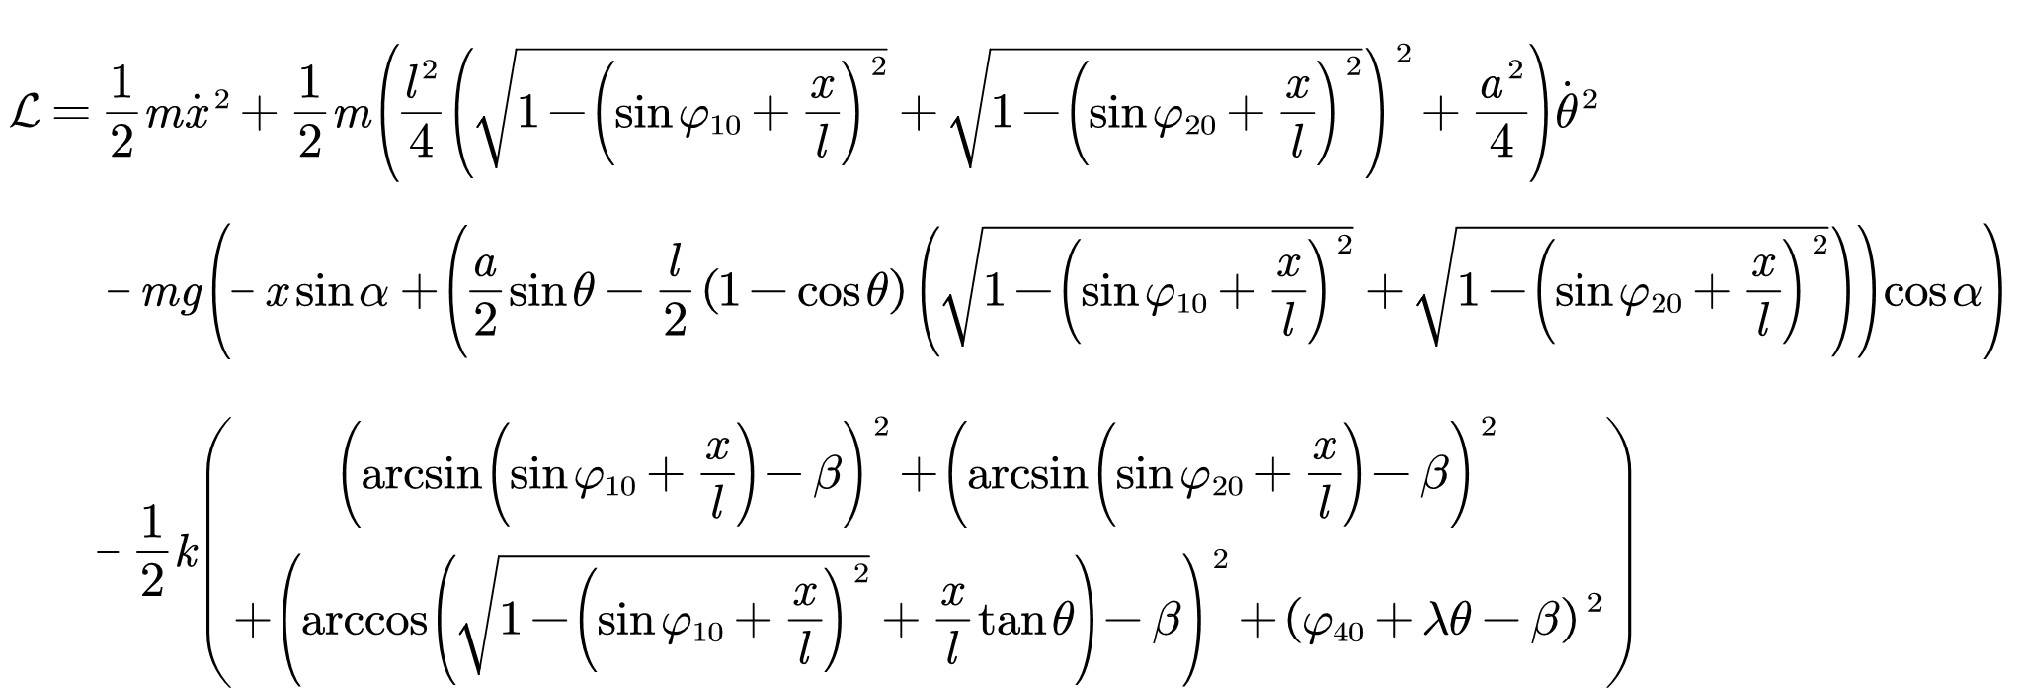
\includegraphics[width=1.1\linewidth]{LagrangeComplex}
				\caption*{}
				\label{fig:lagrangecomplex}
			%\end{adjustbox}
		\end{figure}
	\end{frame}
	
	\begin{frame}
		\begin{figure}
			\centering
			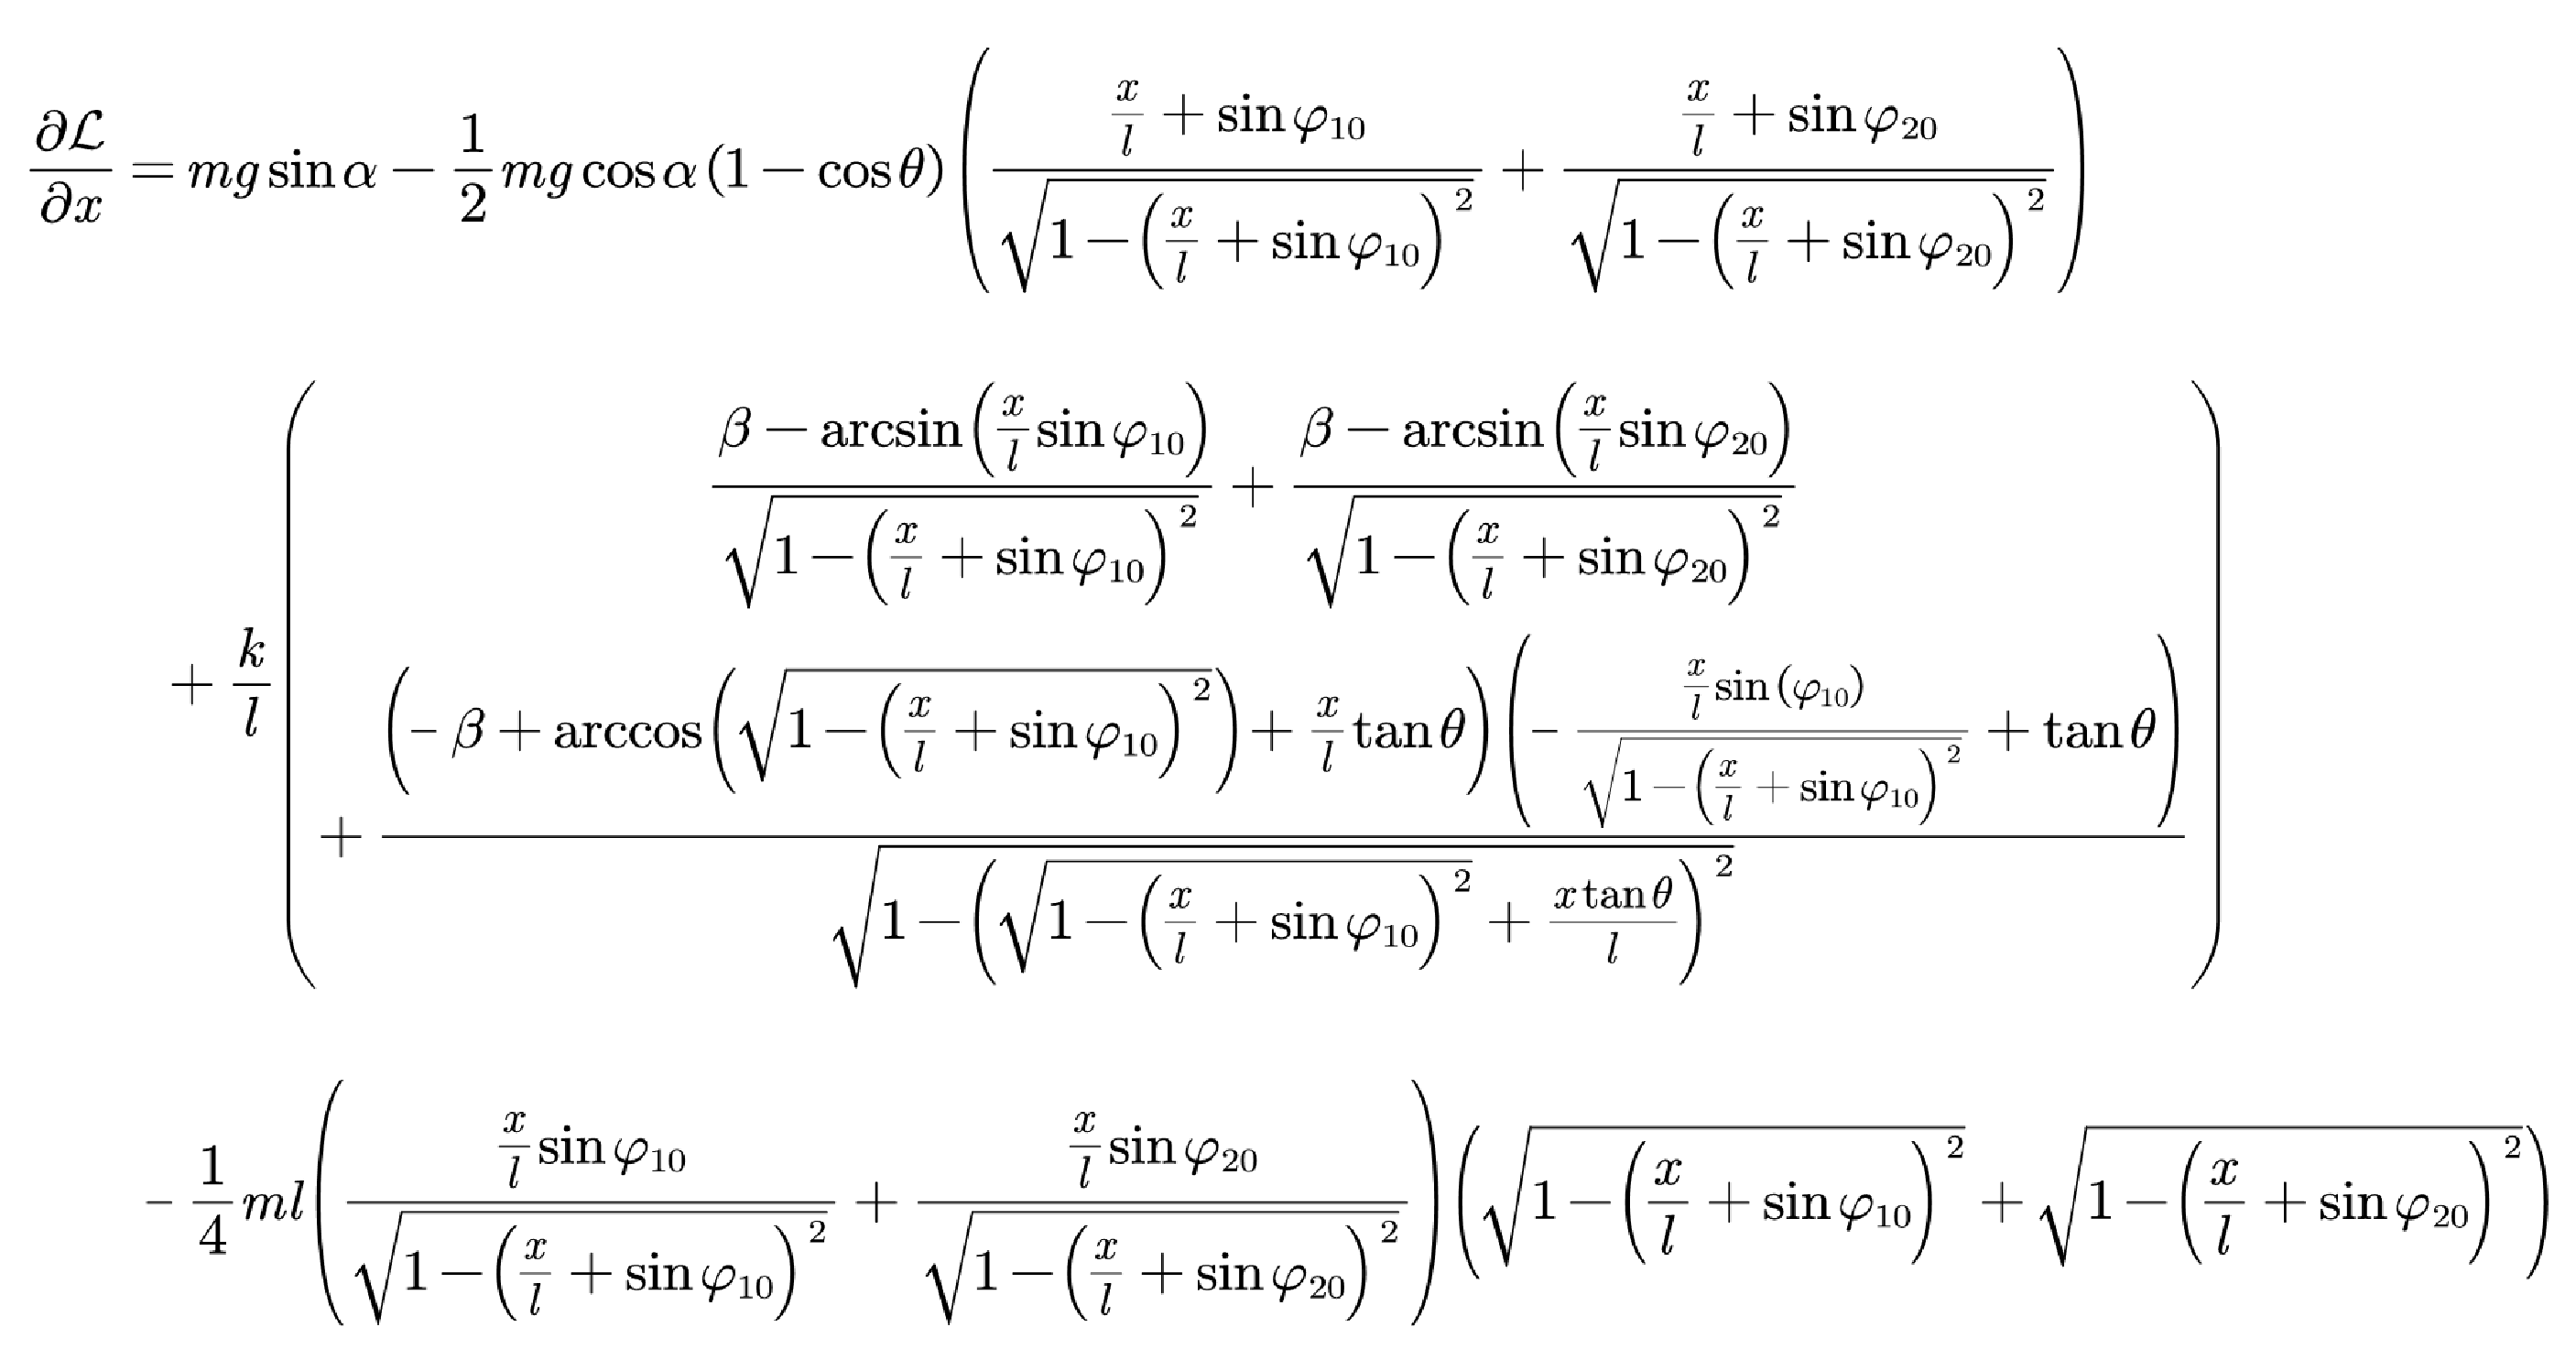
\includegraphics[width=1.1\linewidth]{PartialLOverPartialX}
			\caption*{}
			\label{fig:partialloverpartialx}
		\end{figure}
	\end{frame}
	
	\begin{frame}
		\begin{figure}
			\centering
			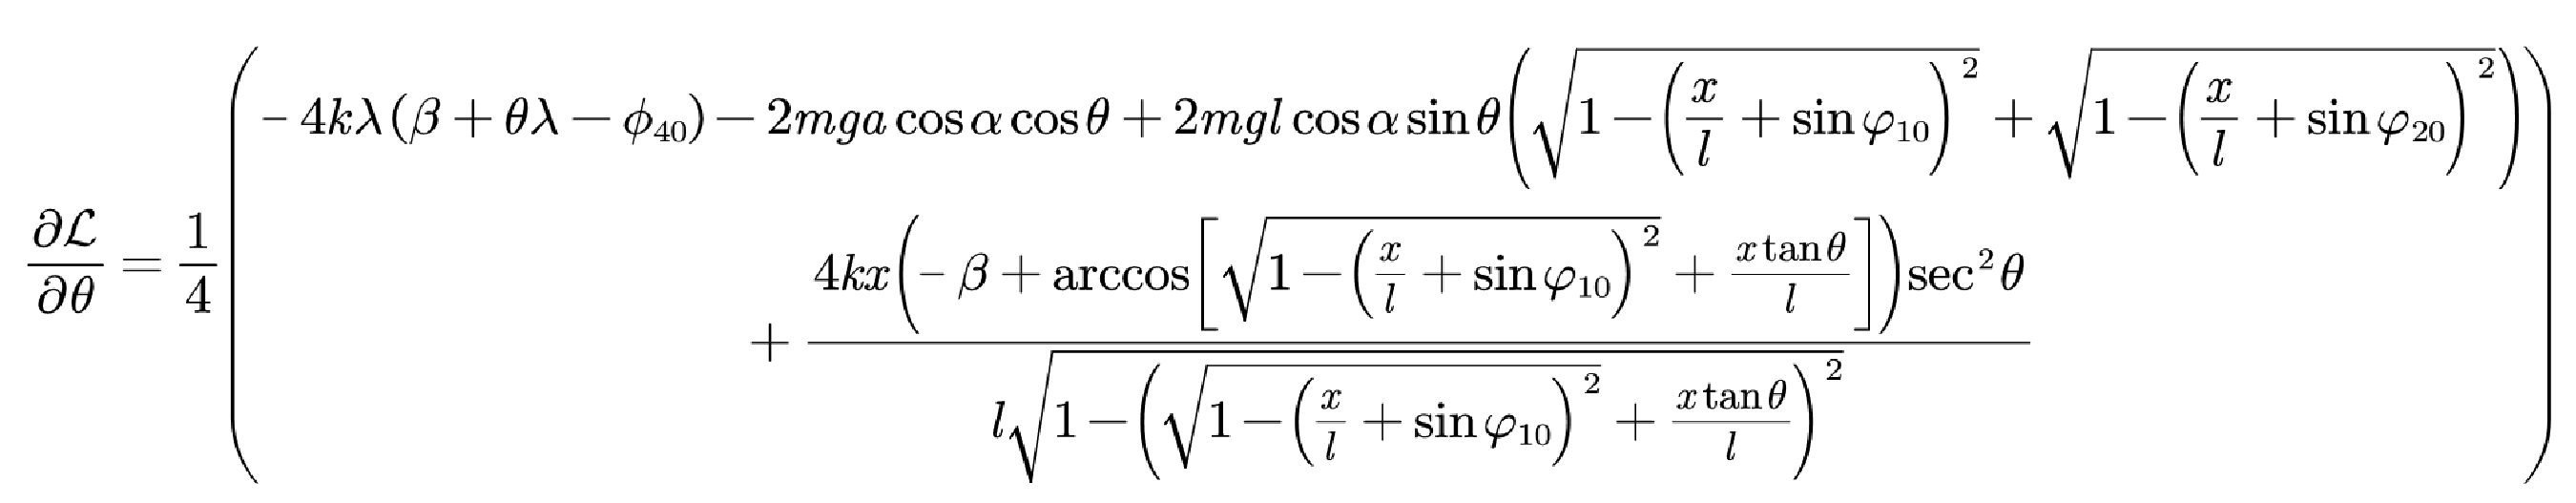
\includegraphics[width=1.1\linewidth]{PartialLOverPartialTheta}
			\caption*{}
			\label{fig:partialloverpartialtheta}
		\end{figure}
	\end{frame}
	
	\begin{frame}
		\begin{small}
			$$
			\frac{\partial\mathcal{L}}{\partial \dot{x}}=m\dot{x}
			$$
			$$
			\frac{\partial\mathcal{L}}{\partial \dot{\theta}}=m\left( \frac{a^2}{4}+\frac{1}{4}l^2\left( \sqrt{1-\left( \frac{x}{l}+\sin \varphi _{10} \right) ^2}+\sqrt{1-\left( \frac{x}{l}+\sin \varphi _{20} \right) ^2} \right) ^2 \right) \dot{\theta}
			$$
			$$
			\frac{\mathrm{d}}{\mathrm{d}t}\frac{\mathcal{L}}{\partial \dot{x}}=m\ddot{x}
			$$
			\begin{align*}
				\frac{\mathrm{d}}{\mathrm{d}t}\frac{\mathcal{L}}{\partial \dot{\theta}}=&m\left( \frac{a^2}{4}+\frac{1}{4}l^2\left( \sqrt{1-\left( \frac{x}{l}+\sin \varphi _{10} \right) ^2}+\sqrt{1-\left( \frac{x}{l}+\sin \varphi _{20} \right) ^2} \right) ^2 \right) \ddot{\theta}
				\\
				&-\frac{1}{2}ml^2\left( \sqrt{1-\left( \frac{x}{l}+\sin \varphi _{10} \right) ^2}+\sqrt{1-\left( \frac{x}{l}+\sin \varphi _{20} \right) ^2} \right)
				\\
				 &\cdot\left( \frac{\left( \dfrac{x}{l}+\sin \varphi _{10} \right) \dfrac{\dot{x}}{l}}{\sqrt{1-\left( \dfrac{x}{l}+\sin \varphi _{10} \right) ^2}}+\frac{\left( \dfrac{x}{l}+\sin \varphi _{20} \right) \dfrac{\dot{x}}{l}}{\sqrt{1-\left( \dfrac{x}{l}+\sin \varphi _{20} \right) ^2}} \right) \dot{\theta}
			\end{align*}
			
		\end{small}
	\end{frame}
	
	\begin{frame}
		\frametitle{关于广义坐标$x$的Lagrange方程}
		把上面算完的关于$x$各项代入Euler-Lagrange方程
		\begin{figure}
			\centering
			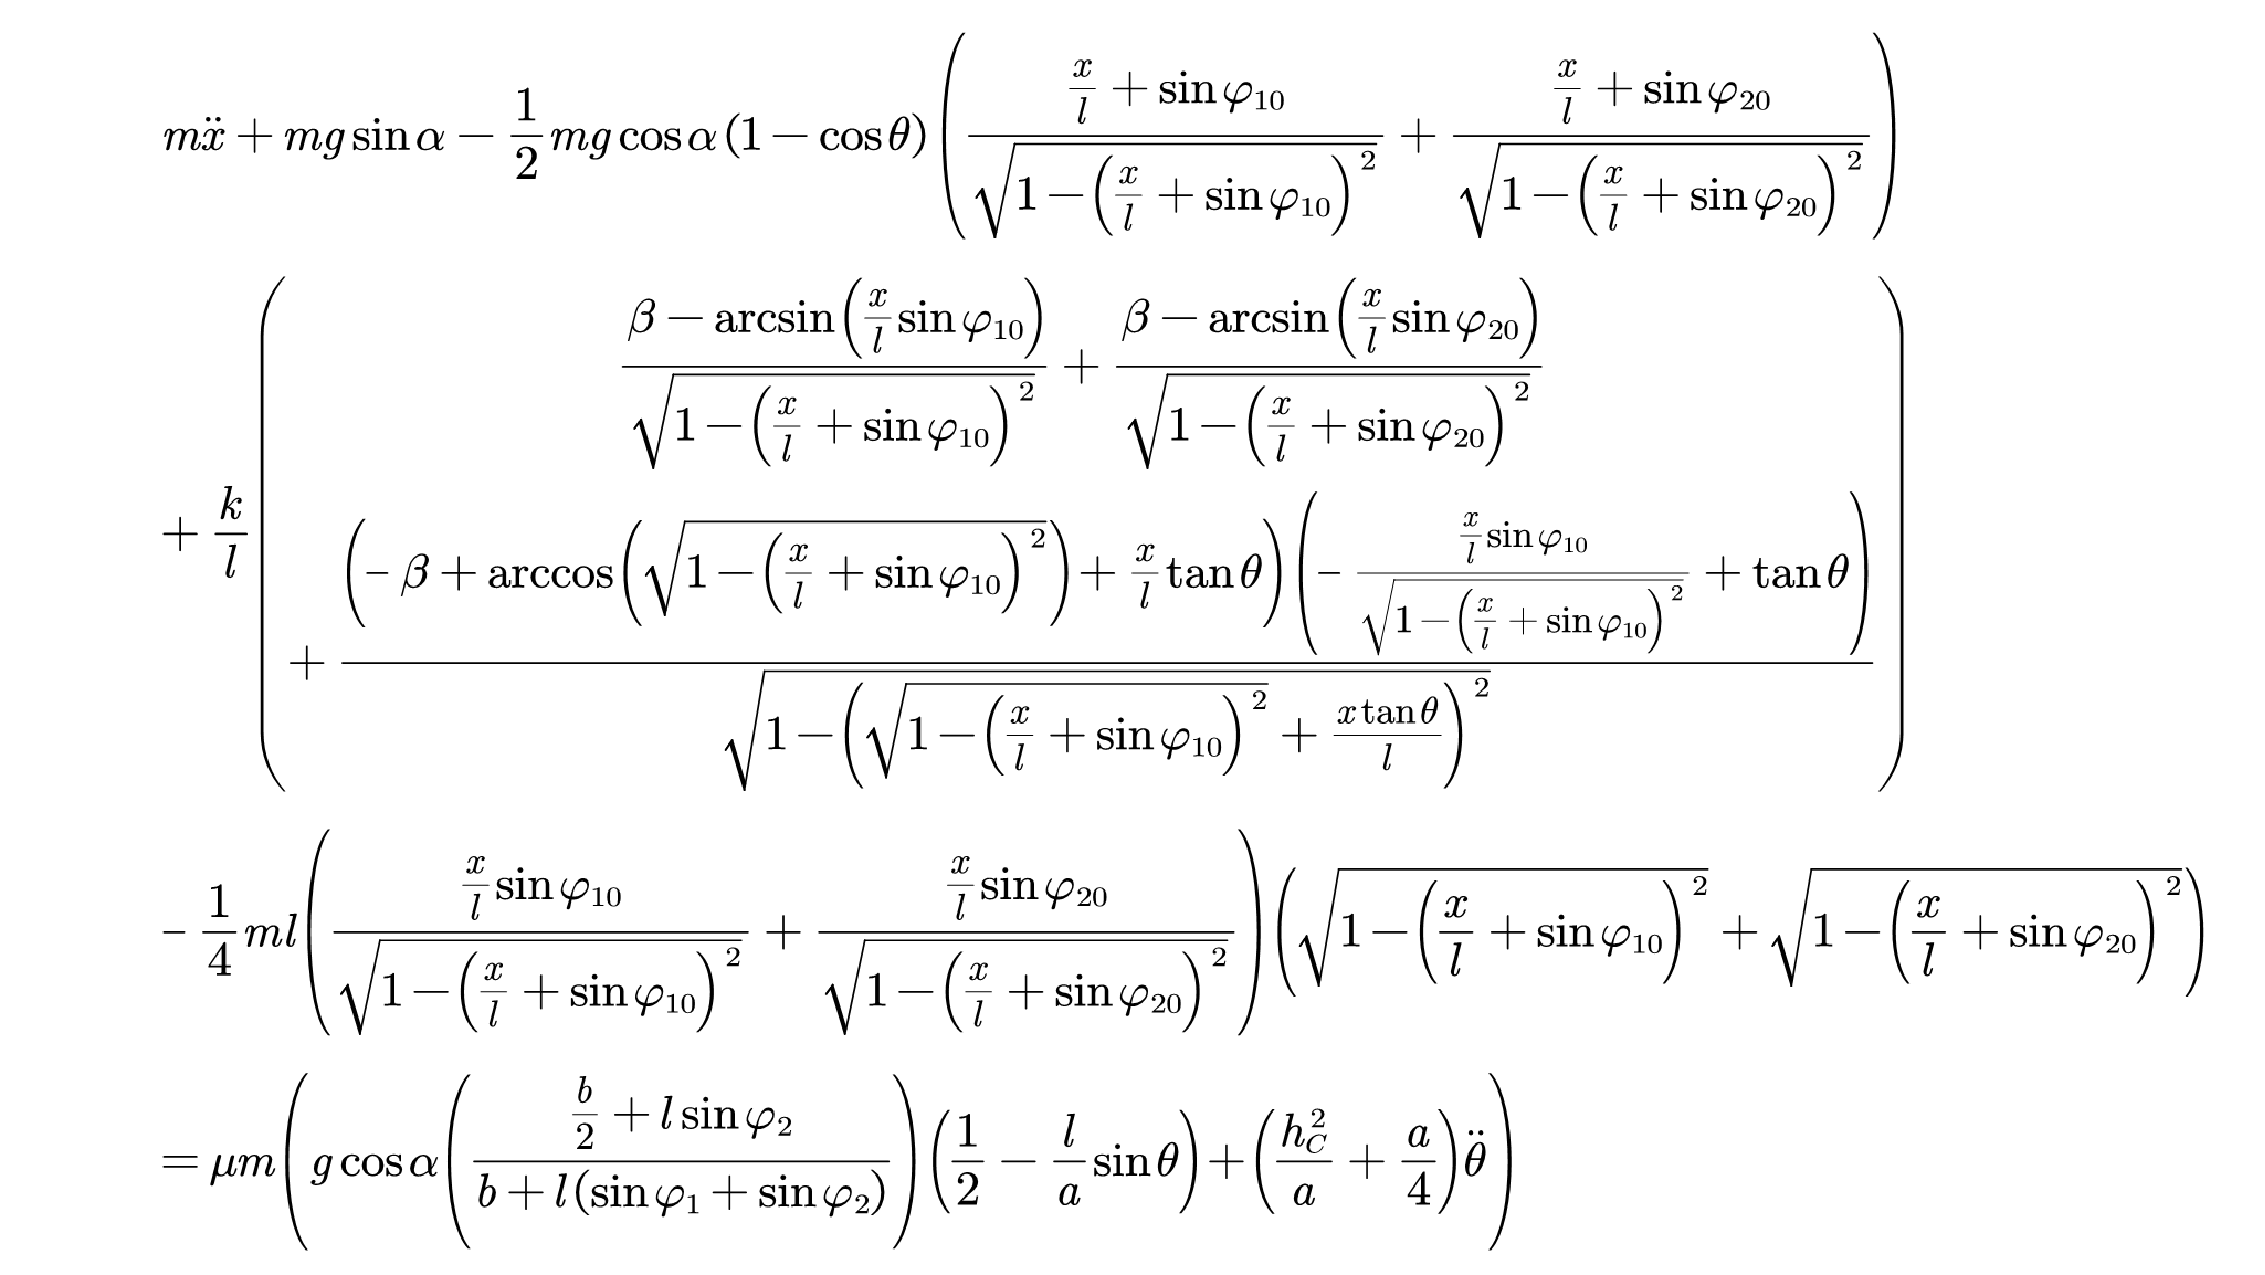
\includegraphics[width=1.1\linewidth]{FirstLagrangeEquationOfX}
			\caption*{}
			\label{fig:firstlagrangeequationofx}
		\end{figure}
	\end{frame}
	
	\begin{frame}
		\frametitle{关于广义坐标$\theta$的Lagrange方程}
		\begin{figure}
			\centering
			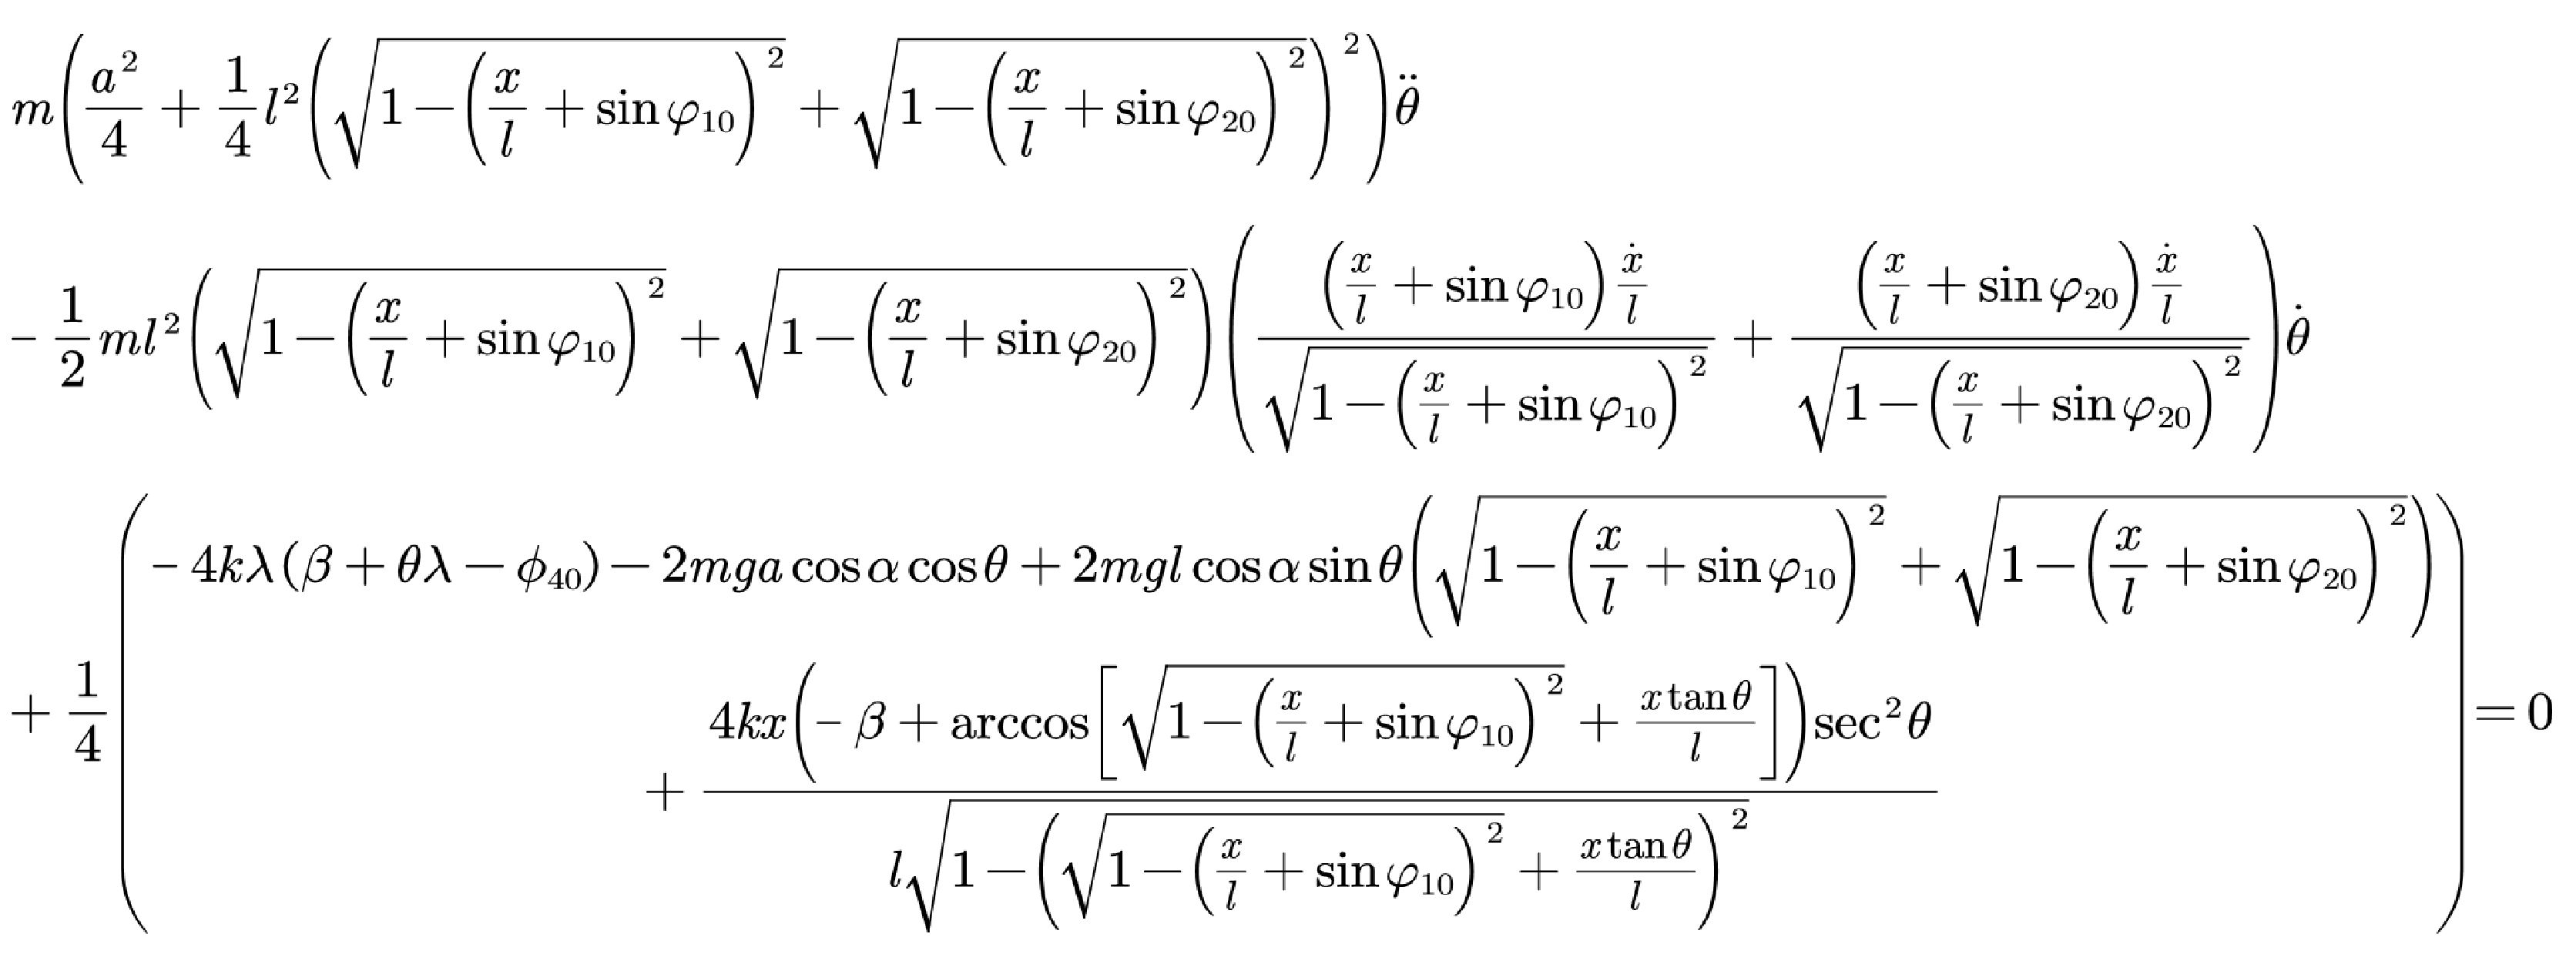
\includegraphics[width=1.1\linewidth]{SecondLagrangeEquationOfTheta}
			\caption*{}
			\label{fig:secondlagrangeequationoftheta}
		\end{figure}
	\end{frame}
	
	\section{代码实现}
	\begin{frame}[plain,c]
		\begin{center}
			\Huge 代码实现
		\end{center}
	\end{frame}
	
	\begin{frame}
		\frametitle{方程常微分化}
		由于原来的方程过于复杂,就算适当化简也会因为微分方程中含有不可分离的耦合项(例如对于$\ddot{\theta}$的超越方程不能分离其)而导致不能用solve\_ivp的方法求解,为此我提出以下简化的方法:
		\vspace{1em}$$  $$
		\huge{方程常微分化}
	\end{frame}
	
	\begin{frame}
		\frametitle{$\theta$的常微分化方程}
		由于$x$相对身体的尺度是小量,不妨对于$\theta$及其导数而言,如果前面的系数中含$x$则直接视作常数,对于不可分离的变元,不妨直接视作常数,即忽略耦合的贡献,那么关于$\theta$的微分方程可写作
		$$
		A\ddot{\theta}-B\dot{\theta}+C\theta-D=0
		$$
		其中$A, B, C, D$的解析表达式在关于$\theta$的Lagrange方程中求得,通过模拟实验我们可以给出一组参考值。
		
		$A=7.7\times10^{-4}, B=7.53\times10^{-5}, C=5.6, D=0.17$
	\end{frame}
	
	\begin{frame}
		\frametitle{$\theta$常微分化后的数值解}
		模拟实验给出稳定步态时候有$t=0$时$\theta=0 ,\dot{\theta}=2$, solve\_ivp给出的数值解为
		\begin{figure}
			\centering
			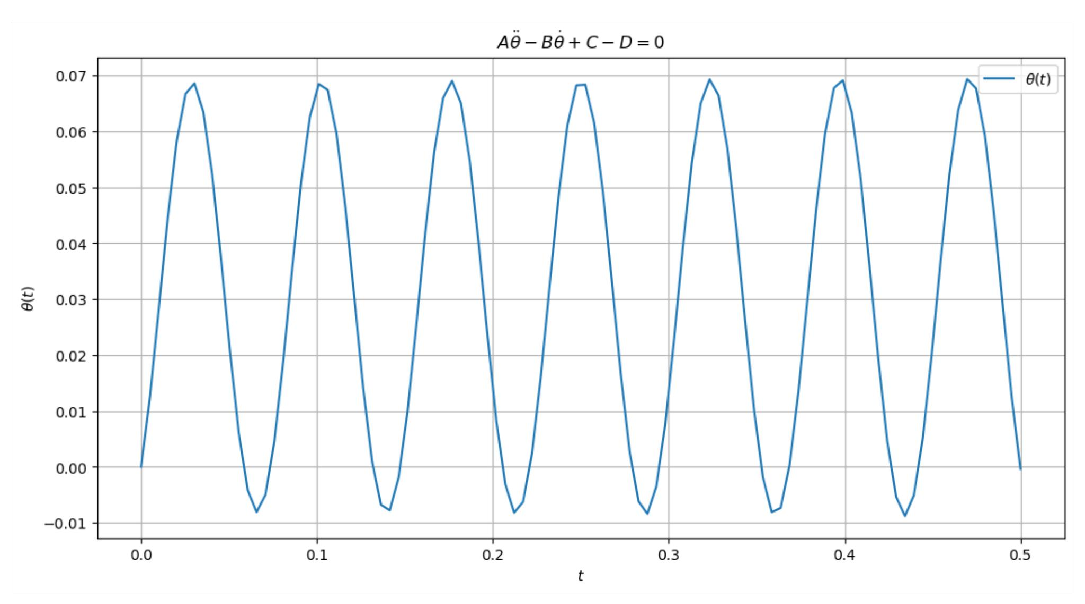
\includegraphics[width=0.9\linewidth]{ThetaNumSolve}
			\caption*{}
			\label{fig:thetanumsolve}
		\end{figure}
		注意这是一次步态的方程对应的解,在$\theta<0$的阶段会失去正常的物理意义
	\end{frame}
	
	\begin{frame}
		\frametitle{步态衔接修正}
		当完成一次步态($\theta=0$,方向从正到负)后,有
		$$
		\theta^+=0\qquad\dot{\theta}^+=2\mathrm{sign}(\dot{\theta}^-)\qquad(\mathrm{sign}\text{表示取符号})
		$$
		\begin{figure}
			\centering
			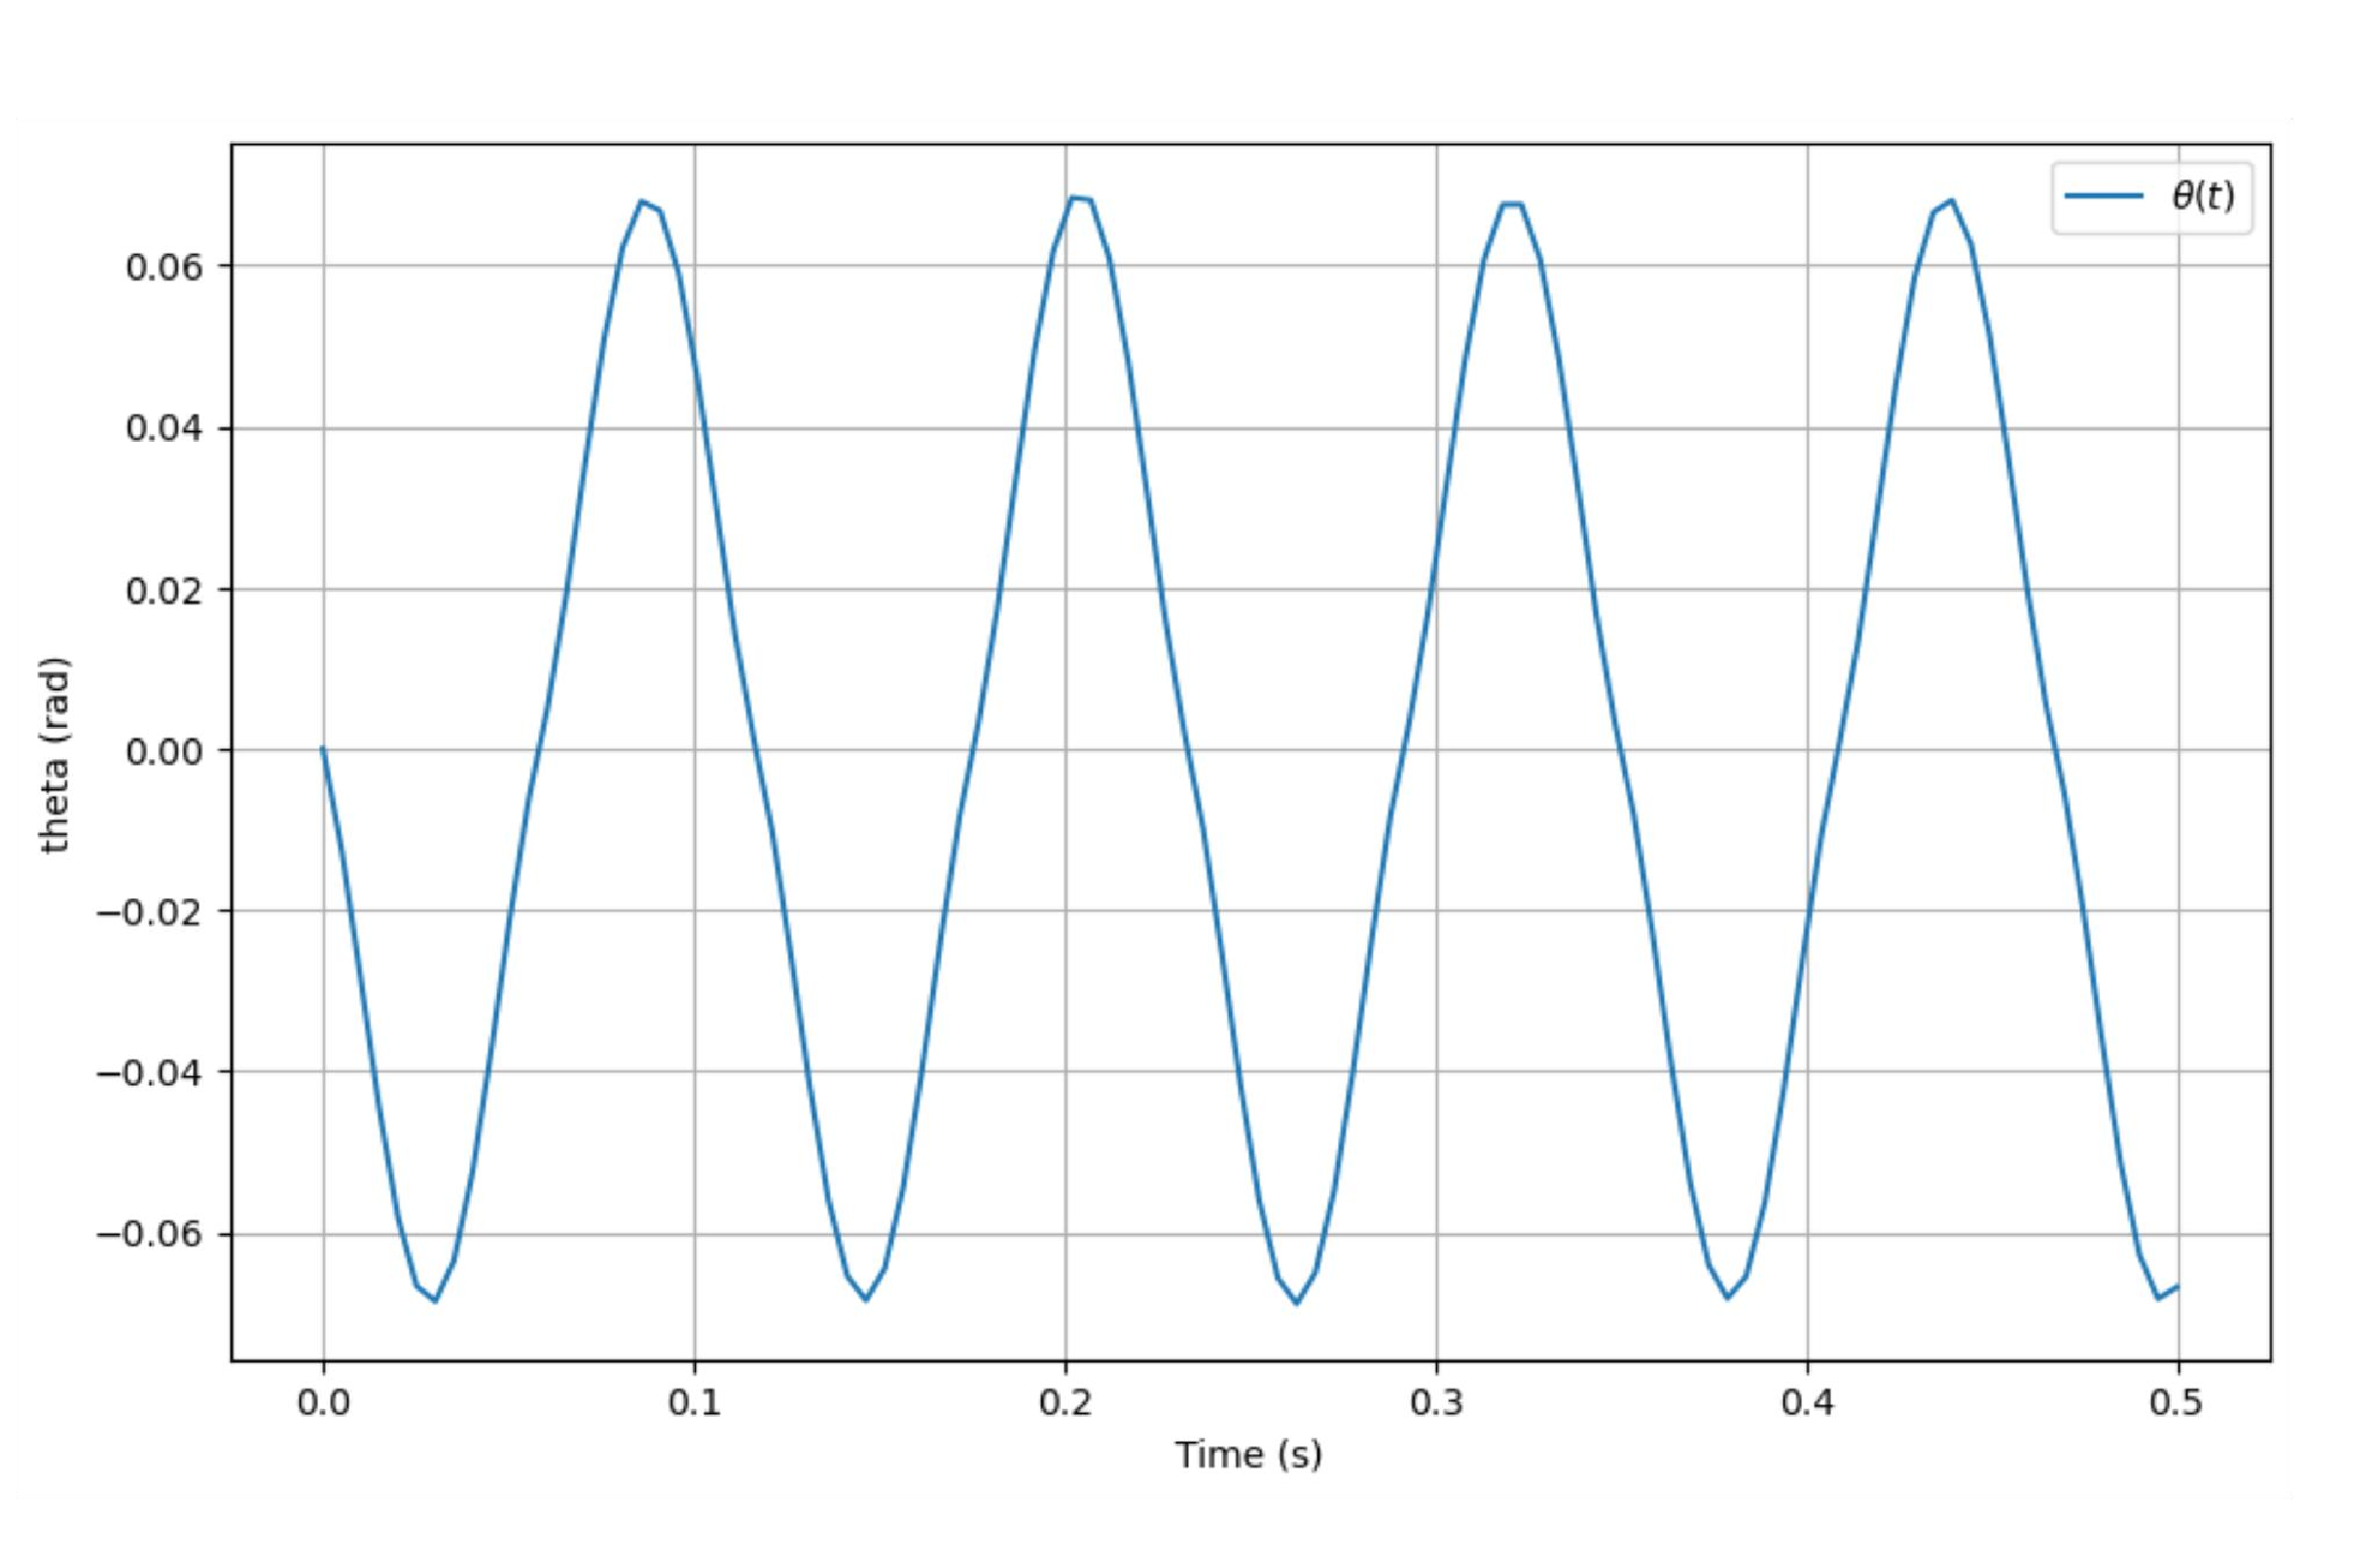
\includegraphics[width=1\linewidth]{FIx}
			\caption*{}
			\label{fig:fix}
		\end{figure}
		
	\end{frame}
	
	%%%%%%%%%%%%%%%%%%%%%%%%%%%%%%%%%%%%%%%%%%%%%%%%%%%%%%%%%%%%%%%%%%%%%%%%%%%%%%%%%%%%	frame}Lastname, Firstname. Year. "Article Title." Journal Name volume (issue): page range. DOI or URL.
	
	\appendix
	\begin{frame}[plain,c]
		\begin{center}
			\Huge 附录
		\end{center}
	\end{frame}
	\begin{frame}{参考文献}
		\begin{thebibliography}{99} % 最大可能的参考文献编号宽度,可以根据实际情况调整
			\bibitem[Author et al., 2021]{ref1}
			[1]Garcia, Mariano, Anindya Chatterjee, Andy Ruina, and Michael Coleman. 1998. "The Simplest Walking Model: Stability, Complexity, and Scaling." ASME Journal of Biomechanical Engineering. Accepted April 16, 1997; final version February 10, 1998.
		\end{thebibliography}
	\end{frame}
	
	
	\begin{frame}
		\frametitle{参考数据(一组有代表性的)}
		\begin{align}
			a&=0.075,&&\phi0=[0.2, 0, 0, 0]\nonumber
			\\
			b&=0.1, &&\beta=0.3\nonumber
			\\
			l&=0.075, &&k=0.04\nonumber
			\\
			\lambda&=1, &&\alpha=0.4\nonumber
			\\
			m&=0.02, &&M=0.05\nonumber
		\end{align}
	\end{frame}
	
	\begin{frame}
		\frametitle{源代码}
		未加入步态衔接修正
		\begin{figure}
			\centering
			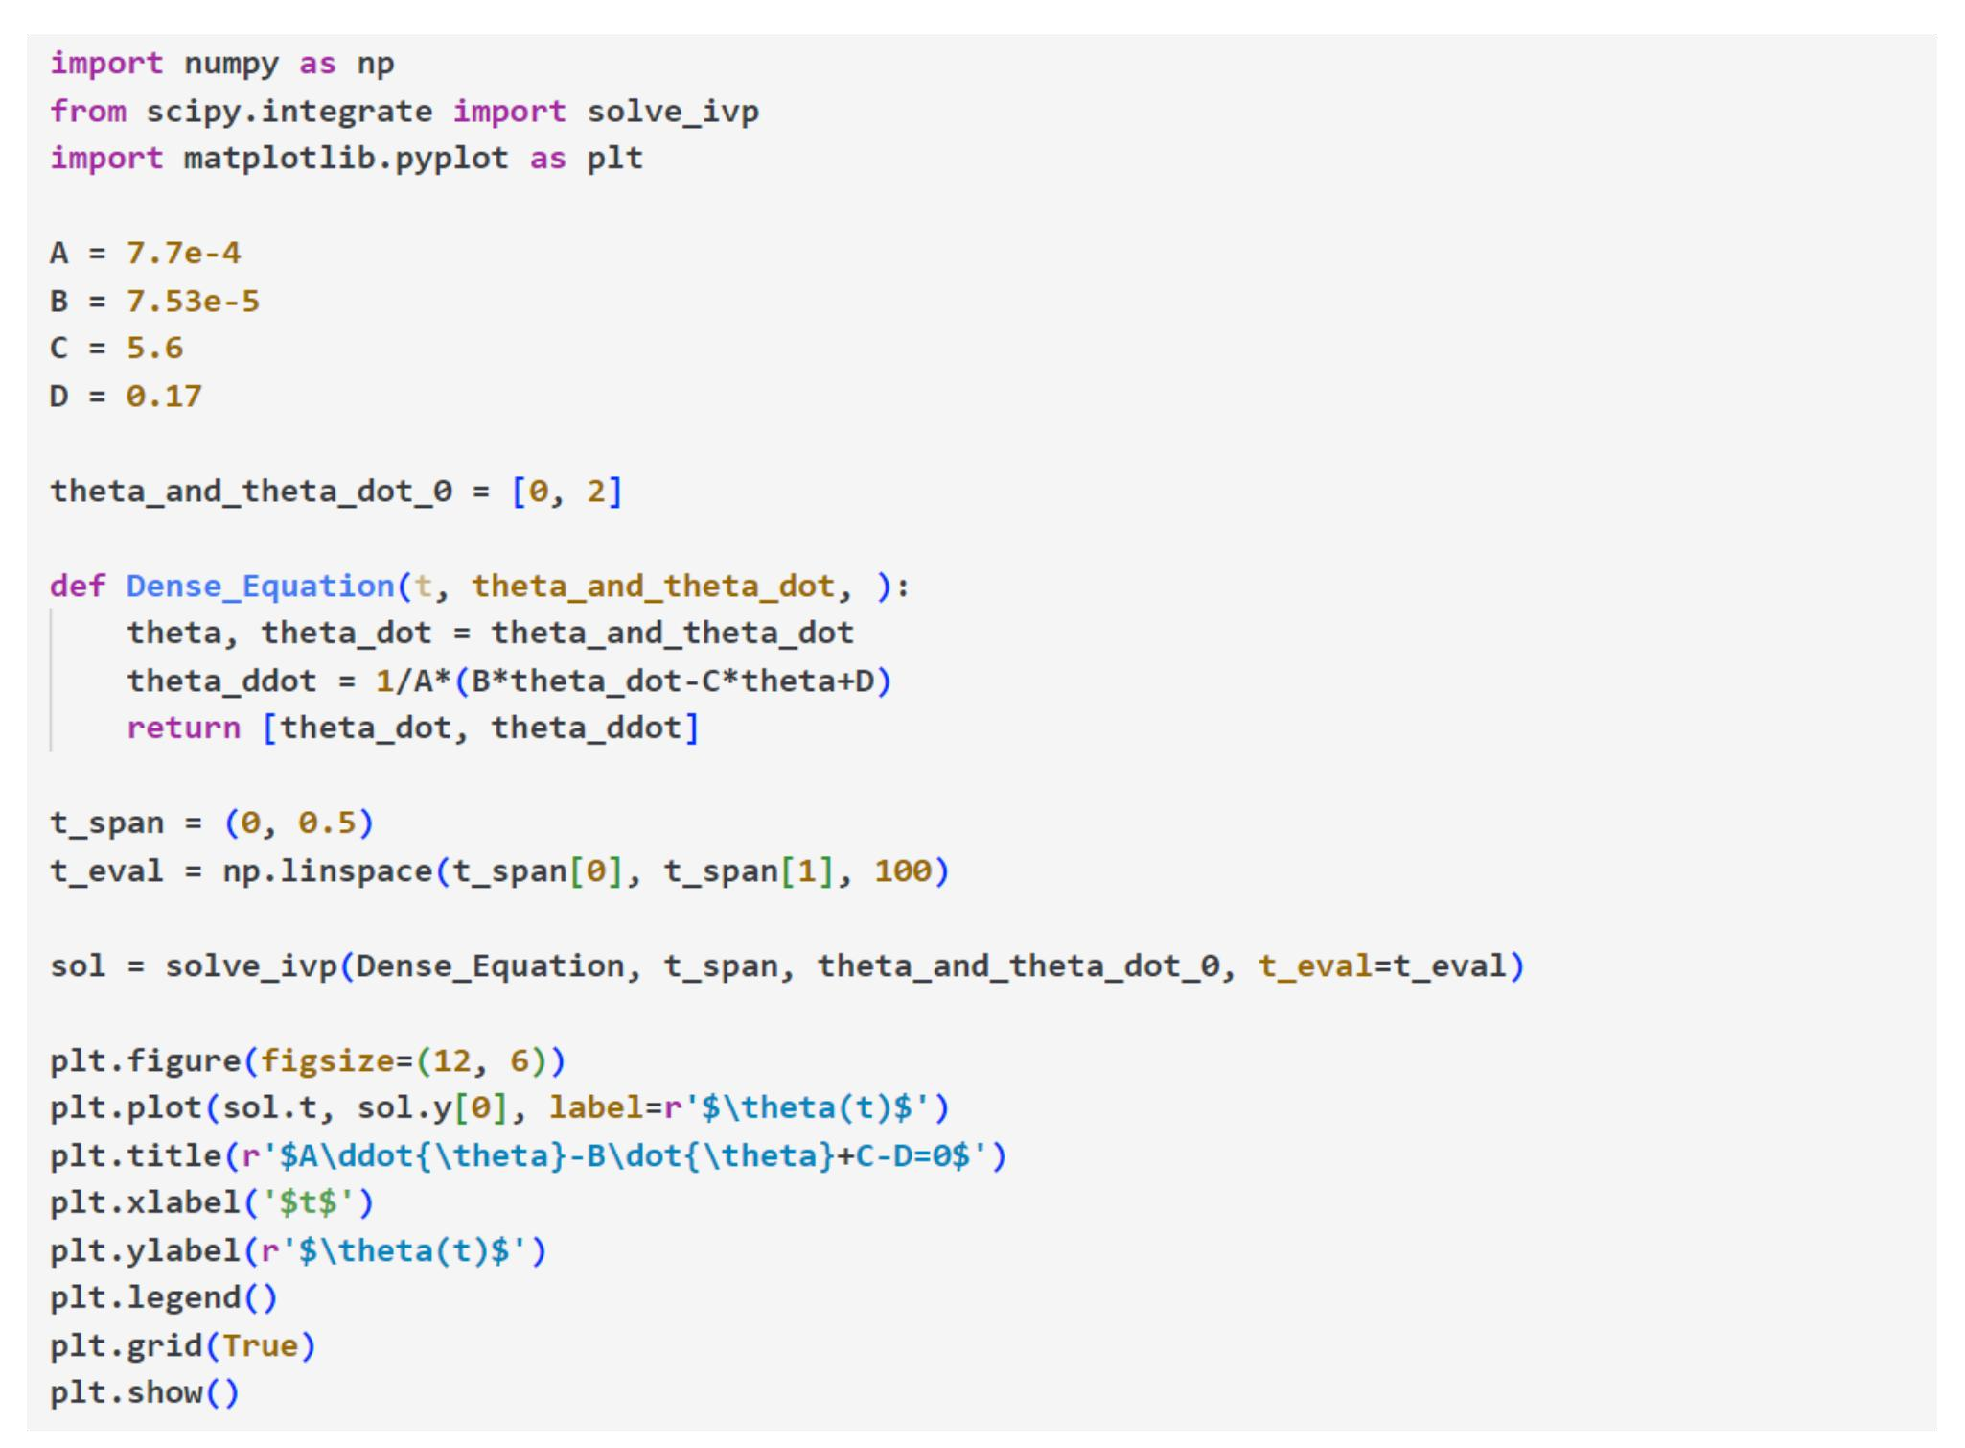
\includegraphics[width=1\linewidth]{Code}
			\caption*{}
			\label{fig:code}
		\end{figure}
	\end{frame}
	
	\begin{frame}
		\frametitle{源代码}
		加入步态衔接修正,利用solve\_ivp的事件监测功能
		\begin{figure}
			\centering
			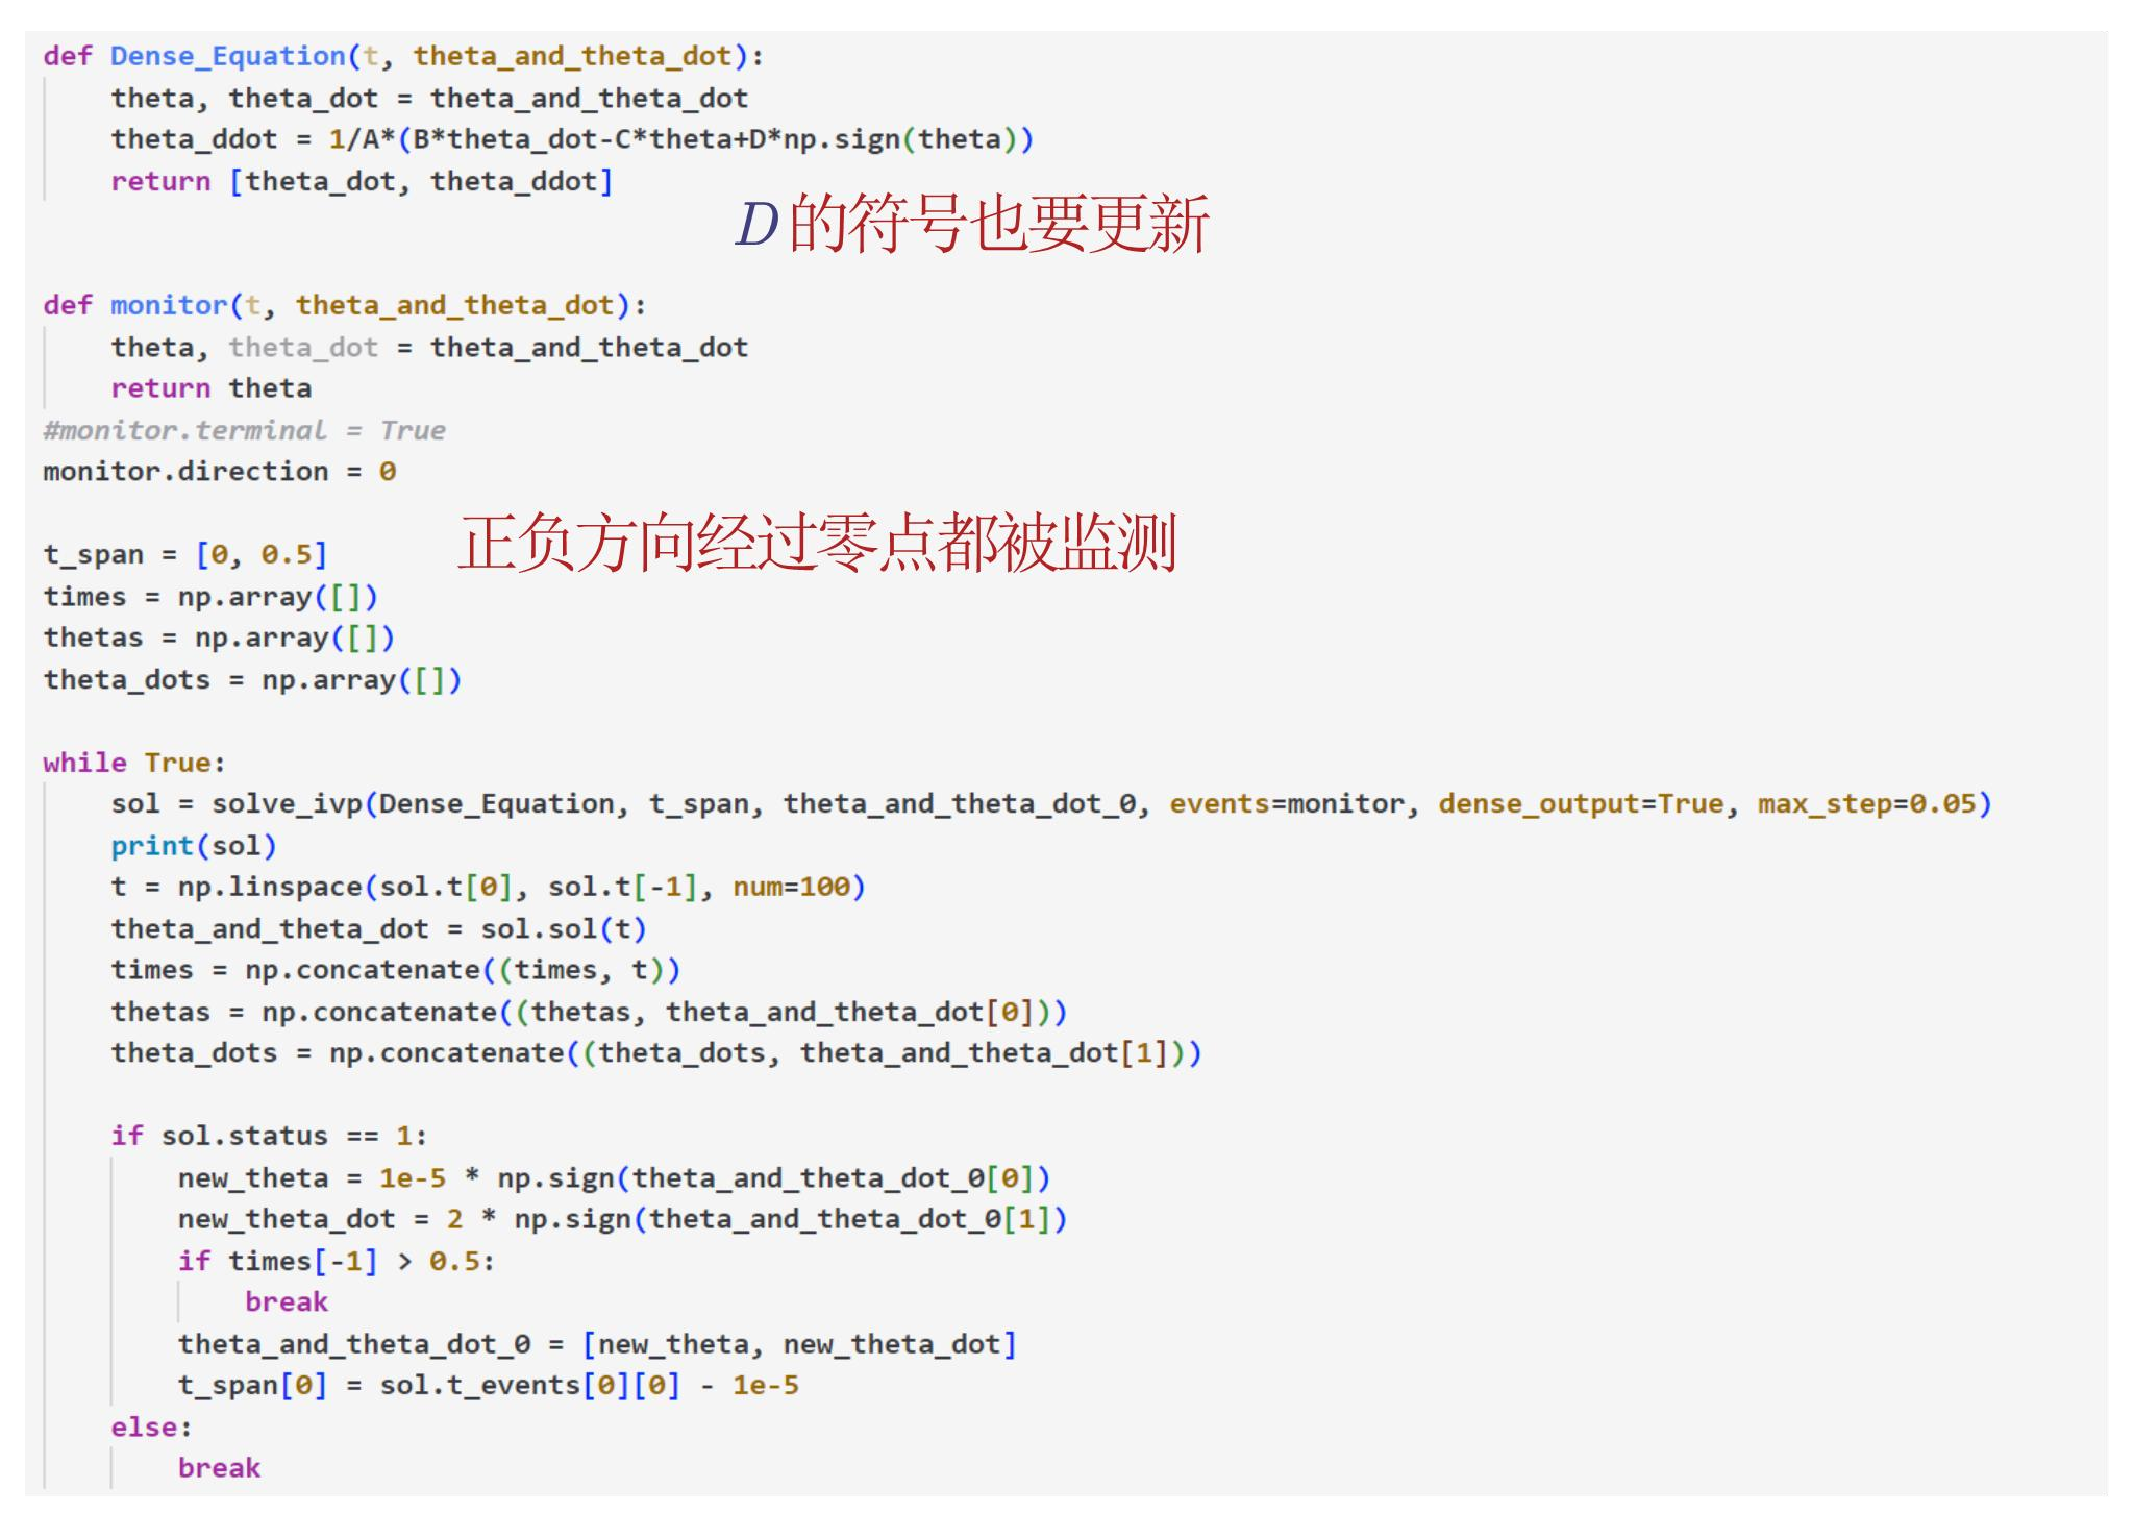
\includegraphics[width=1\linewidth]{CodeNew}
			\caption*{}
			\label{fig:codenew}
		\end{figure}
		
	\end{frame}
	
	\begin{frame}[plain,c]
		\begin{center}
			\Huge END
		\end{center}
	\end{frame}
	
	\end{document}